\documentclass{article}
\usepackage{graphicx} % Required for inserting images
\usepackage[a4paper, margin=2.5cm]{geometry}
\usepackage{amsmath}
\usepackage{float}
\usepackage{tikz}
\usetikzlibrary{arrows.meta, positioning}

\title{INF266 - Problem Set 4}
\author{Ragnil Klete, Maija Evenssssen, Halvard Håvardsrud}
\date{\today}


\begin{document}

\maketitle

\section*{Part I - Problems}
\subsection*{Exercise 1}

\[
\mathcal{M} = (\mathcal{S}, \mathcal{A}, P, R, \gamma)
\]

\paragraph{States}
\[
\mathcal{S} = \{ s_0, s_1, s_2, s_3, s_4, s_5, s_6, s_7 \}
\]
\[
\begin{aligned}
s_0&:\text{empty},\quad
s_1:\text{full},\quad
s_2:\text{sugared},\quad
s_3:\text{salted},\\
s_4&:\text{sugar sampling},\quad
s_5:\text{salt sampling},\\
s_6&:\text{baked sugary},\quad
s_7:\text{baked salty}
\end{aligned}
\]

\paragraph{Actions}
\[
\begin{aligned}
\mathcal{A}(s_0)&=\{\text{wait}, \text{prep}\},\\
\mathcal{A}(s_1)&=\{\text{wait}, \text{sugar}, \text{salt}\},\\
\mathcal{A}(s_2)&=\mathcal{A}(s_3)=\{\text{taste}, \text{cook}, \text{restart}\},\\
\mathcal{A}(s_4)&=\mathcal{A}(s_5)=\{\text{cook}, \text{return}\},\\
\mathcal{A}(s_6)&=\mathcal{A}(s_7)=\emptyset
\end{aligned}
\]

\paragraph{Transitions (deterministic)}
\[
P(s'|s,a)=1 \text{ for:}
\]
\[
\begin{aligned}
&(s_0,\text{wait})\to s_0,\ (s_0,\text{prep})\to s_1\\
&(s_1,\text{sugar})\to s_2,\ (s_1,\text{salt})\to s_3\\
&(s_2,\text{taste})\to s_4,\ (s_2,\text{cook})\to s_6,\ (s_2,\text{restart})\to s_1\\
&(s_3,\text{taste})\to s_5,\ (s_3,\text{cook})\to s_7,\ (s_3,\text{restart})\to s_1\\
&(s_4,\text{cook})\to s_6,\ (s_4,\text{return})\to s_2\\
&(s_5,\text{cook})\to s_7,\ (s_5,\text{return})\to s_3
\end{aligned}
\]

\paragraph{Reward}
\[
R(s,a,s') =
\begin{cases}
+10 & s' = s_6\\
-10 & s' = s_7\\
0 & \text{otherwise}
\end{cases}
\]

\[
\gamma \in [0,1]
\]
\newpage
\subsection*{Exercise 2}
\begin{figure}[h]
    \centering
    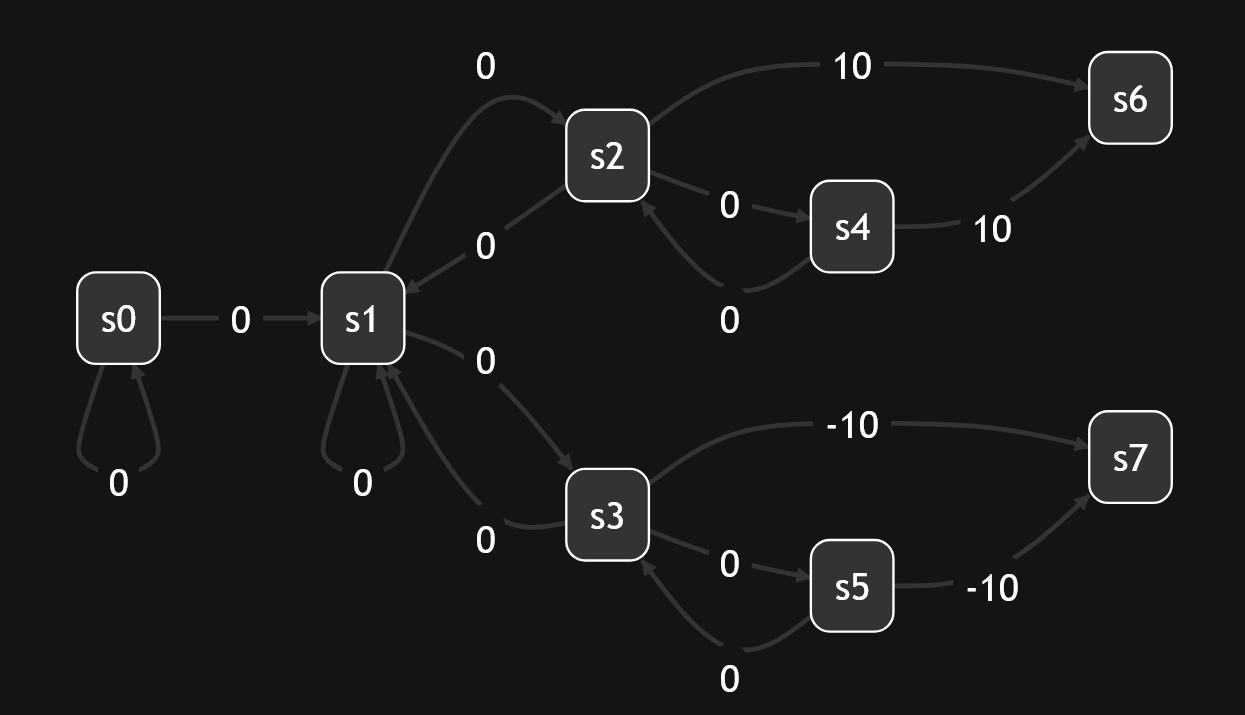
\includegraphics[width=1\textwidth]{diagram.png}
    \caption{Backup diagram for the MDP.}
\end{figure}

\subsection*{Exercise 3}
\begin{textbf}
    yes, we can define an optimal deterministic policy for this MDP. The optimal policy would be:
    \begin{enumerate}
        \item In state $s_0$, take action \text{prep} to move to state $s_1$.
        \item  In state $s_1$, take action \text{sugar} to move to state $s_2$.
        \item In state $s_2$, take action \text{cook} to move to state $s_6$ and receive a reward of +10.
    \end{enumerate}
    This policy is optimal because it leads to the highest possible reward of +10 by reaching state $s_6$.
    Any deviation from this policy would either lead to a lower reward (e.g., going to state $s_7$ with a reward of -10), a delayed reward (like taking action \text{taste} in $s_2$ leading to state $s_4$), or no reward at all (e.g., waiting in state $s_0$ or taking the restart action in states $s_2$ or $s_3$). Therefore, the optimal deterministic policy is to always choose the actions that lead to state $s_6$.
    This policy is simply the shortest path to the highest reward.
\end{textbf}

\subsection*{Exercise 4}
\begin{textbf}
    
\end{textbf}

\end{document}